\section{Results}

\begin{table}[ht]
\caption{
    \textbf{Benchmark Results.} Test accuracy of all methods on \texttt{TM} and \texttt{SP} in the 5-way-5-shot setting. We depict the average accuracy and the 95\% confidence interval both without (left) and with SOT (right) and the difference.
    \vspace{5pt}
}

\label{tab:tuned-benchmark}
\centering
\begin{tabular}{llllr}
\toprule
 &  & \multicolumn{2}{@{}c}{\textbf{Test Acc. (\%)}} & \\
 &  & w/o SOT & w/ SOT & Diff \\
\midrule
\multirow[c]{5}{*}{\texttt{TM}} & B & $90.7 \pm 0.7$ & $86.3 \pm 0.9$ & {\color{red} +4.8} \\
 & B++ & $81.9 \pm 0.9$ & $82.8 \pm 0.9$ &  {\color{teal} +1.1} \\
 & MAML & $\mathbf{92.8} \pm 0.5$ & $99.2 \pm 0.1$ & {\color{teal} +6.9} \\
 & MN & $84.6 \pm 0.8$ & $\mathbf{99.7} \pm 0.1$ &  {\color{teal} +17.9} \\
 & PN & $87.1 \pm 0.8$ & $98.6 \pm 0.2$ & {\color{teal} +13.2} \\
\midrule
\multirow[c]{5}{*}{\texttt{SP}} & B & $\mathbf{69.2} \pm 0.7$ & $55.7 \pm 0.8$ & {\color{red} -19.6} \\
 & B++ & $64.1 \pm 0.7$ & $64.6 \pm 0.7$ & {\color{teal} +0.8} \\
 & MAML & $68.7 \pm 0.7$ & $98.0 \pm 0.2$ & {\color{teal} +42.8} \\
 & MN & $68.2 \pm 0.8$ & $\mathbf{99.8} \pm 0.1$ & {\color{teal} +46.5} \\
 & PN & $63.5 \pm 0.7$ & $99.2 \pm 0.1$ & {\color{teal} +56.1} \\
\bottomrule
\end{tabular}
\end{table}

Figure~\ref{fig:benchmark-perf} and Table \ref{tab:tuned-benchmark} shows the test accuracies for each method with and without the SOT module on both datasets.

% Without SOT:
% TM: (91.3 + 81.7 + 89.8 + 85.3 + 90)/5 = 87.6
% SP: (69.1 + 55.2 + 61.5 + 65.4 + 64.3)/5 = 63.1
Models without the SOT module reach an average accuracy of 88\% on the \texttt{TM} dataset and 63\% on the \texttt{SP} dataset. These results generally show that the models are capable of learning from few samples, improving significantly over the random baseline of 20\% accuracy. Peak performances in this group are achieved by \texttt{B} on both datasets, with 91\% and 69\% accuracy, respectively.

% With SOT:
% TM: (91.9 + 89.8 + 90.9 + 93.5 + 91.6)/5 = 90.4
% SP: (64.7 + 64.5 + 67.2 + 70.0 + 66.6)/5 = 66.6
Models incorporating the SOT module exhibit enhanced accuracy, achieving 90\% and 67\% average accuracy on the \texttt{TM} and \texttt{SP} dataset. All models benefit from the inclusion of the SOT feature transform module, except for \texttt{B} on \texttt{SP}. 

Notably, \texttt{MN} on \texttt{SP} demonstrates the most significant gain with SOT: from a lowest accuracy of 55\% to the highest at 70\%. The addition of the SOT module increases the peak accuracy by 0.9 percentage points on \texttt{SP} and 2.2 on \texttt{TM}.

\begin{figure}[h!]
    \centering
    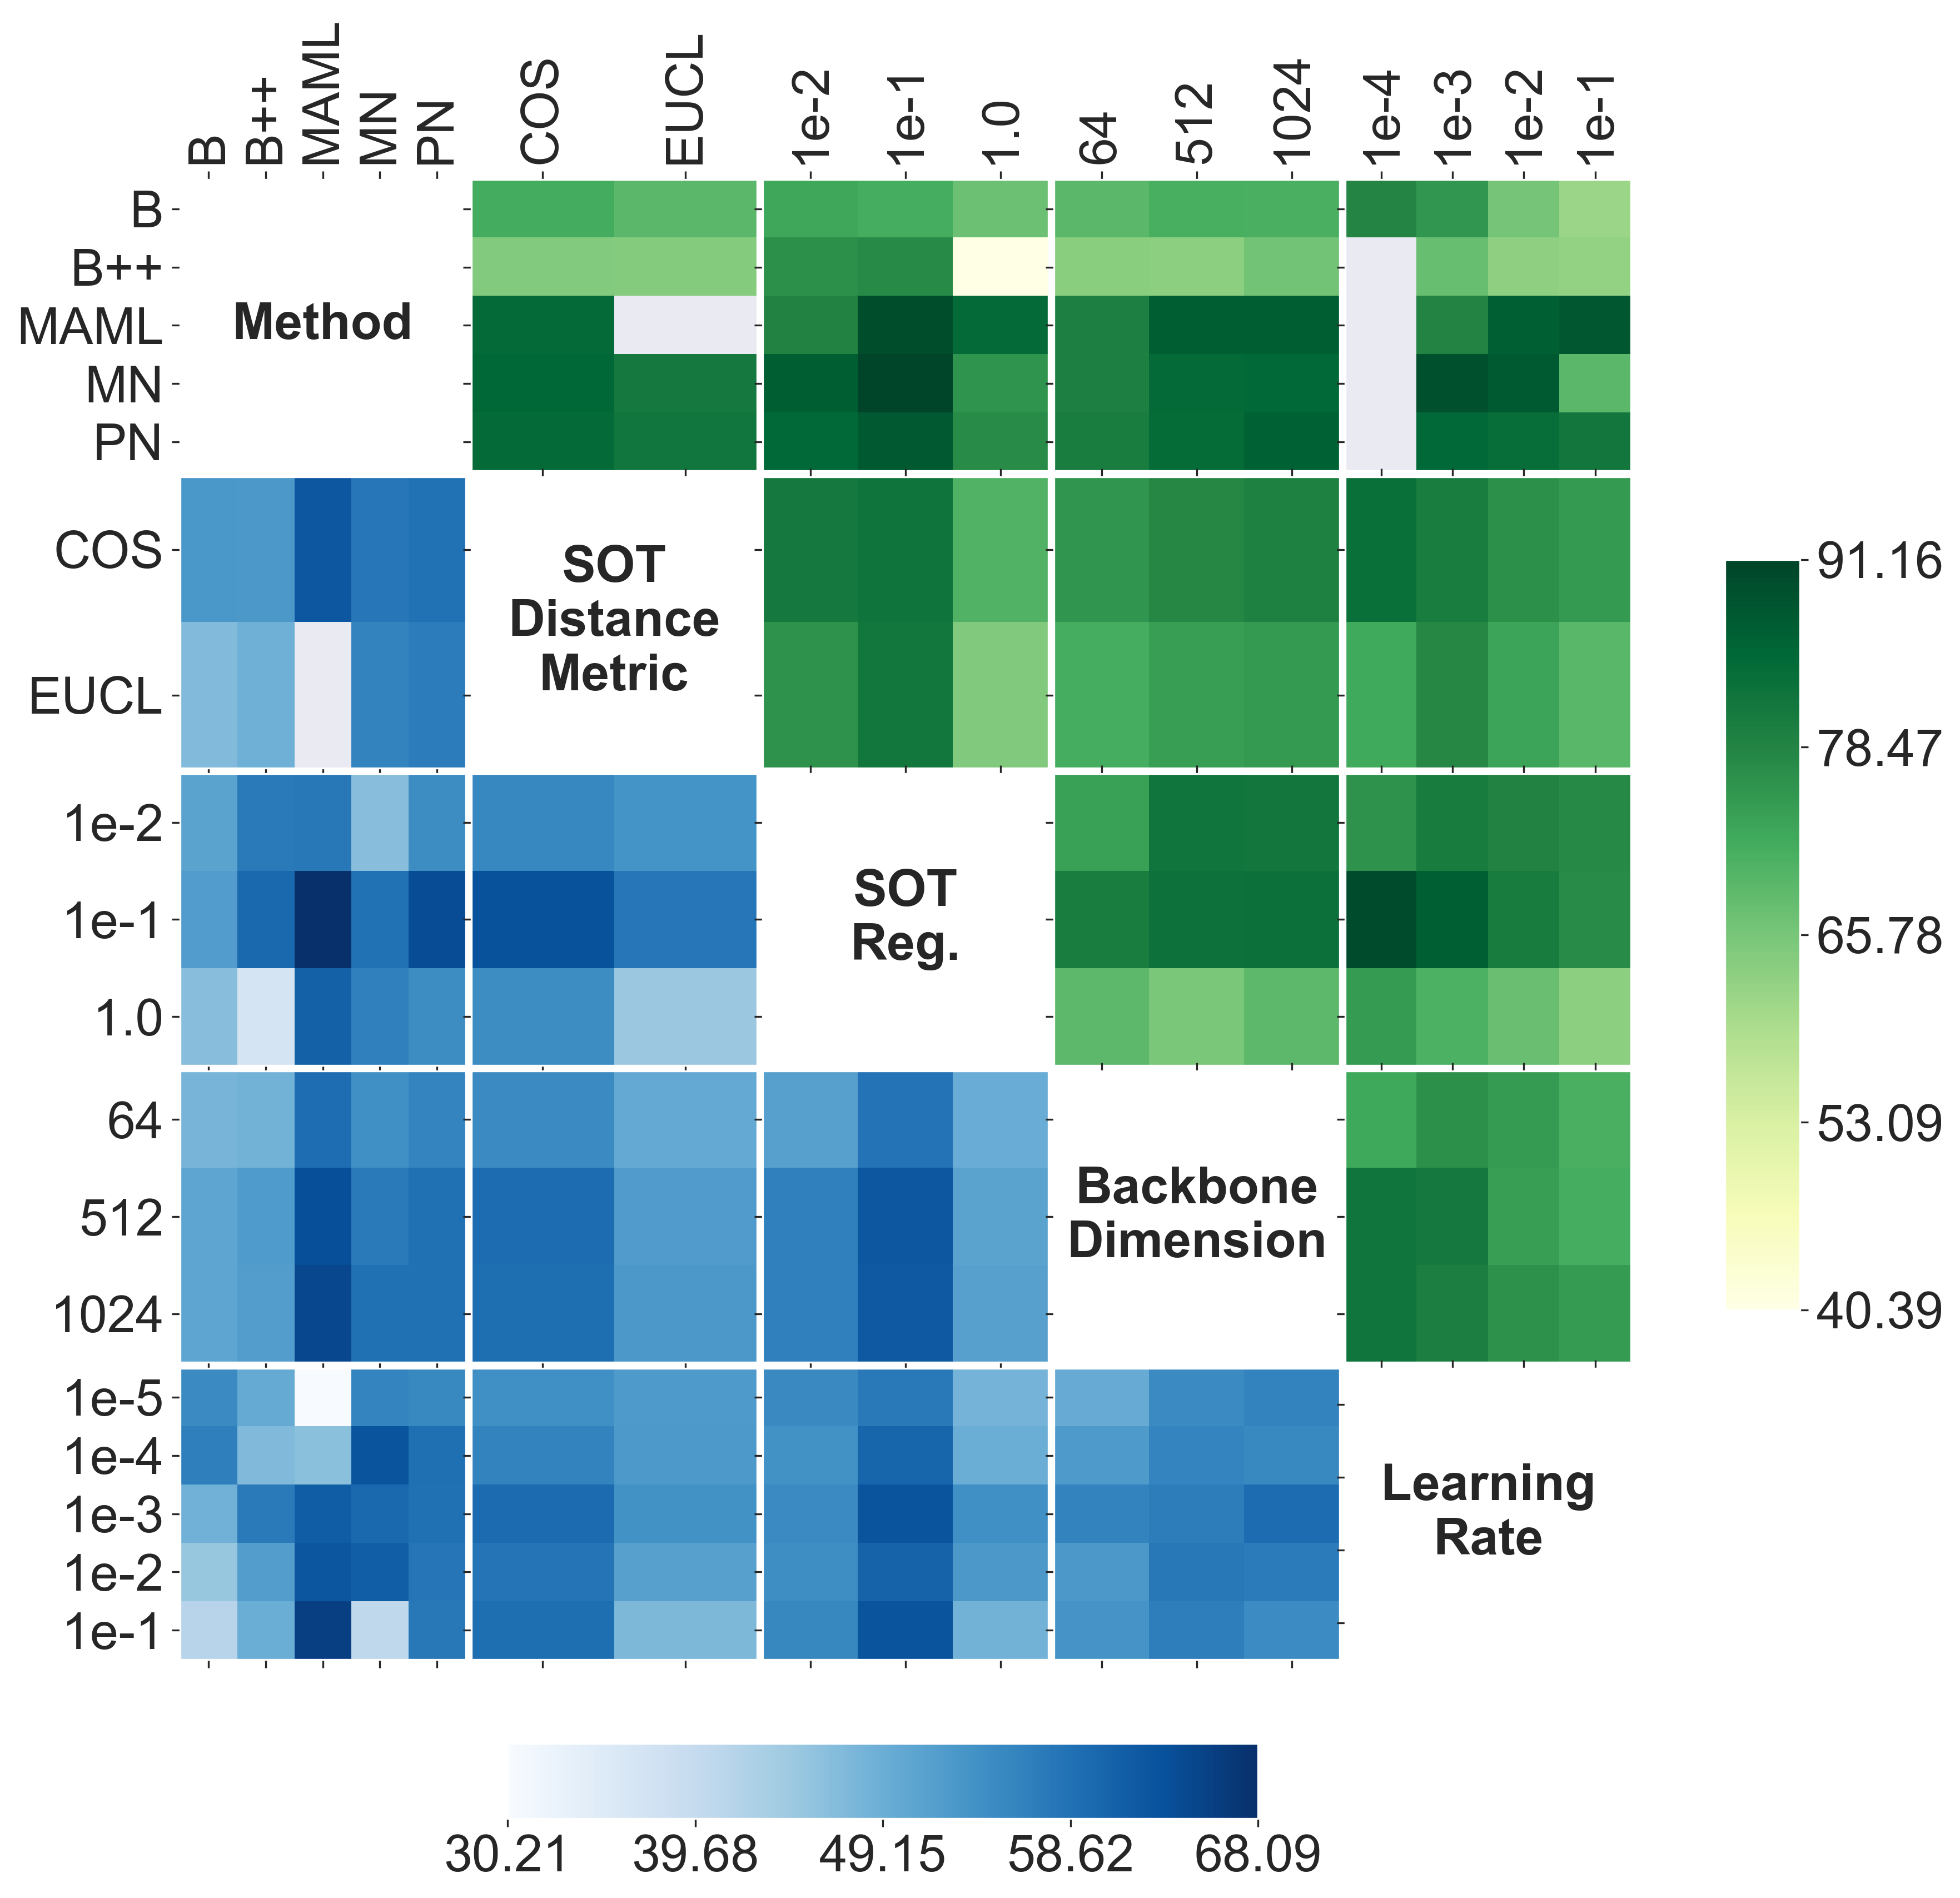
\includegraphics[width=1\columnwidth]{figures/hparams-interaction-combined.png}
    \caption{\textbf{Hyperparameter Ablation.} Average test accuracies on the \texttt{SP} dataset for all pairs of hyperparameter settings for \texttt{SP} in blue (bottom left) and \texttt{TM} in green (top right).}
    \label{fig:hparams-swissprot-grid}
\end{figure}

\textbf{Hyperparameter Ablation.} Figure~\ref{fig:hparams-swissprot-grid} shows the pair-wise interactions between all tuned hyperparameters for both datasets separately. We add a column for the methods to study how they react to certain hyperparameters configurations. 

The plots indicate a clear trend across all methods and datasets regarding the SOT hyperparameters: We find that using the cosine distance metric and regularisation with $\gamma = 0.1$ consistently yields the best performance. 
Furthermore, we find that the choice of the learning rate has a significant impact on the performance of all methods. \texttt{B}, \texttt{B++} and \texttt{MN} generally prefer lower learning rates of $\lambda=1e^{-4}$, while \texttt{MAML} prefers high learning rates of $\lambda=1e^{-1}$. \texttt{PN}'s performance is robust to the choice of learning rate showing no significant variation across tuning runs.
Finally, the plot reveals that \texttt{MN}, \texttt{PN}, and \texttt{MAML} are generally more robust to the choice of hyperparameters, yielding higher mean accuracies across tuning runs, while  \texttt{B++} was found especially sensitive. Despite being the best performing method on \texttt{SP}, its mean accuracy is lower in the tuning runs.



\textbf{Way-Shot Analysis.} Figure~\ref{fig:way-shot} illustrates \texttt{PN}'s way-shot analysis on the TM dataset, comparing scenarios with and without the SOT module. The left subplot depicts test accuracy versus the number of classes (ways), while the right subplot relates accuracy to the number of samples per class (shots). In both SOT and non-SOT contexts, a consistent trend emerges: accuracy diminishes linearly with more classes and grows with additional samples per class up to some limit. Notably, exceeding ten samples per class yields no substantial accuracy gains. As expected, the model's performance with the SOT module is consistently higher for higher numbers of classes and samples.

\begin{figure}[h!]
    \centering
    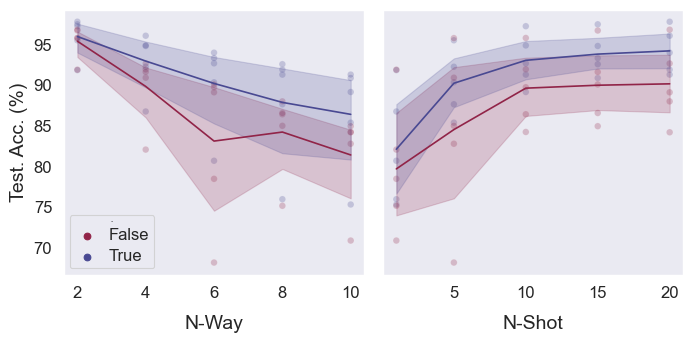
\includegraphics[width=1\columnwidth]{figures/way-shot.png}
    \caption{\textbf{Way-Shot Analysis.} Test accuracy of \texttt{PN} on the \texttt{TM} dataset with and without the SOT module in various 
    few-shot learning settings for fixed n-way (left) and n-shot (right). Individual points represent a single experiment. We show the regression line with a 95\% confidence interval.}
    \label{fig:way-shot}
\end{figure}
